\section{Estimación de estado}
La estimación de estado consiste en determinar el estado no medible de un sistema dinámico a partir de las mediciones de entrada y salida de dicho sistema, esto es, dado un estado inicial $\bm{x}_0$ y las observaciones $\bm{y}_1, \bm{y}_2, ..., \bm{y}_k$ conocidas en el tiempo $k$, el problema de estimación de estado en el paso de tiempo $k$ se basa en construir un estimador $\hat{\bm{x}}_k$ de $\bm{x}_k$.

Lamentablemente, las mediciones no son perfectas, lo que conduce a una inexactitud inherente en el valor de la medición. Para tener en cuenta estos errores, la estimación de estado procesa todas las mediciones disponibles y utiliza un \textit{análisis de regresión} para identificar el estado real probable del sistema.

\subsection{Filtro de Kalman}
El filtro de Kalman es un filtro Gaussiano con transición de estado y función de medición \textit{lineales}. Se le atribuye a {\big[\textbf{Kalman, 1960}]} y {\big[\textbf{Swerling, 1958}]} y se ha aplicado por primera vez al seguimiento por radar de objetivos aéreos, pero se ha utilizado en una gran cantidad de otros problemas de estimación desde entonces. El filtro de Kalman y sus diversos derivados son casi ubicuos en las aplicaciones de fusión de sensores.

El objetivo de este filtro, entonces, es computar $\{\hat{\bm{x}}_k,\hat{\bm{P}_k}\}$ utilizando toda la información disponible, incluyendo la presente en el tiempo $k$. Mientras el método de cuadrados mínimos recursivo actualiza la estimación de un parámetro estático, el filtro de Kalman es capaz de actualizar la estimación de un estado en evolución. Como se deriva del filtro general de Bayes{\Big[\textbf{REF BAYES}]}, el objetivo de este filtro es tomar una estimación probabilística de este estado y actualizarla en tiempo real usando dos pasos, \textit{predicción} y \textit{corrección}.

Para poder entender mejor el filtro, se considera el problema de estimar la posición de un vehículo en una dimensión. Iniciando de una estimación probabilística en el tiempo $k-1$, el objetivo es predecir el nuevo estado mediante un modelo de moción, el cual puede ser derivado, por ejemplo, de la odometría de las ruedas o de las mediciones de una unidad inercial. Luego, con el modelo de observación derivado de, por ejemplo, los datos del GPS, se corrige esa predicción de la posición del vehículo en el tiempo $k$, tal como se observa en la Figura \ref{fig:kalmanfilter}. Cada una de estas componentes, la estimación inicial, el estado predicho, y el estado final corregido son todas variables aleatorias especificadas por sus valores medios y covarianzas. De este modo, puede pensarse al Filtro de Kalman como una técnica para fusionar información de diferentes sensores para producir una estimación final de un estado desconocido, tomando en cuenta incertidumbres en el moción y en las mediciones\footnote{Para identificar estados predichos de corregidos, por ejemplo en la matriz de covarianza $\bm{P}$, para el primer caso se utiliza la notación $\check{\bm{P}}$, mientras que para el segundo caso $\hat{\bm{P}}$.}.

\begin{figure}
    \centering
    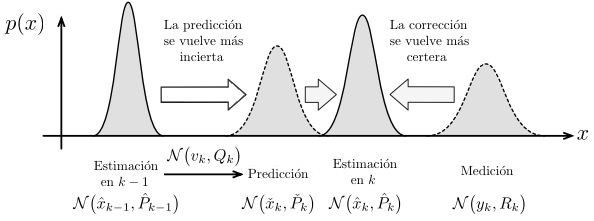
\includegraphics[width=\textwidth]{Img/KalmanFilter.png}
    \caption{Filtro de Kalman en una dimensión}
    \label{fig:kalmanfilter}
\end{figure}

En concreto, el filtro de Kalman requiere de un modelo de moción
\begin{equation}
    \bm{x}_k = \bm{F}_{k-1}\bm{x}_{k-1} + \bm{G}_{k-1}\bm{u}_{k-1} + \bm{w}_{k-1},
\end{equation}
y un modelo de medición lineal
\begin{equation}
    \bm{y}_k = \bm{H}_k\bm{x}_k + \bm{v}_k,
\end{equation}
siendo $\bm{u}_{k-1}$ una \textit{entrada de control} externa que afecta la evolución del estado del sistema, $\bm{v}_{k-1}$ el \textit{ruido de la medición} y $\bm{w}_{k-1}$ el \textit{rudo del proceso} que gobierna la incertidumbre de las entradas de control
\begin{equation}
    \bm{v}_k \sim \mathcal{N}(\bm{0},\bm{R}_k)\hspace{2cm}\bm{w}_k \sim \mathcal{N}(\bm{0},\bm{Q}_k)
\end{equation}

Puede decirse que el filtro de Kalman \textit{es muy similar a un estimador de cuadrados mínimos recursivo que incluye un modelo de moción} el cual indica cómo el estado evoluciona a través del tiempo. El mismo consta de dos pasos
\begin{enumerate}
    \item \textbf{Predicción}. Primero, se utiliza el modelo del proceso o moción para predecir como los estados evolucionaron desde el último paso de tiempo, y se propaga la incertidumbre.
    \begin{align}
        \check{\bm{x}}_k &= \bm{F}_{k-1}\bm{x}_{k-1}+\bm{G}_{k-1}\bm{u}_{k-1} \\
        \check{\bm{P}}_k &= \bm{F}_{k-1}\hat{\bm{P}}_{k-1}\bm{F}_{k-1}^T + \bm{Q}_{k-1}
    \end{align}
    \item \textbf{Actualización}. En el mismo se utiliza el modelo de medición y puede dividirse en dos pasos
    \begin{enumerate}
        \item \textit{Ganancia óptima}. Se utiliza la medición para corregir la predicción basada en el residuo o innovación de la medición y la ganancia óptima
        \begin{equation}
            \bm{K}_k = \check{\bm{P}}_{k}\bm{H}_k^T\left(\bm{H}_k\check{\bm{P}}_k\bm{H}_k^T + \bm{R}_k\right)^{-1}
        \end{equation}
        \item \textit{Corrección}. Se utiliza la ganancia para propagar la covarianza de estado de la predicción a la estimación corregida.
        \begin{align}
            \hat{\bm{x}}_k &= \check{\bm{x}}_k + \bm{K}_k\left(\bm{y}_k - \bm{H}_k\check{\bm{x}}_k\right) \\
            \hat{\bm{P}}_k &= (\bm{1} - \bm{K}_k\bm{H}_k)\check{\bm{P}}_k
        \end{align}
        siendo $(\bm{y}_k - \bm{H}_k\check{\bm{x}}_k)$ la llamada \textit{innovación de la medición}.
    \end{enumerate}
\end{enumerate}

Se dice que un estimador o filtro es \textit{insesgado} (en inglés, \textit{unbiased}) si produce un error promedio de cero para todo paso de tiempo k
\begin{equation}
    E[\hat{p}_k-p_k] = 0
\end{equation}
donde $\hat{p}_k$ denota al valor estimado y $p_k$ al valor verdadero.

Considerando la dinámica de error, siendo el error de estado predicho
\begin{equation}
    \check{\bm{e}}_k = \check{\bm{x}}_k - \bm{x}_k
\end{equation}
y el error de estimación corregido
\begin{equation}
    \hat{\bm{e}}_k = \hat{\bm{x}}_k - \bm{x}_k
\end{equation}
se puede obtener mediante el uso de las ecuaciones del filtro de Kalman que
\begin{align}
    \check{\bm{e}}_k &= \bm{F}_{k-1}\check{e}_{k-1} - \bm{w}_k \\
    \check{\bm{e}}_k &= \left(\bm{1} - \bm{K}_k\bm{H}_k\right)\check{\bm{e}}_k + \bm{K}_k\bm{v}_k
\end{align}

Si se tiene ruido blanco no correlacionado con media cero y
\begin{equation*}
    E[\hat{\bm{e}}_0] = \bm{0}\hspace{0.5cm}\land\hspace{0.5cm}E[\bm{v}] = \bm{0}\hspace{0.5cm}\land\hspace{0.5cm}E[\bm{w}] = \bm{0}
\end{equation*}
se llega a que el valor esperado de estos errores es cero para todo $k$
\begin{align}
    E[\check{\bm{e}}_k] &= \bm{F}_{k-1}E[\check{\bm{e}}_{k-1}] - E[\bm{w}_k] = \bm{0} \\
    E[\hat{\bm{e}}_k] &= \left(\bm{1} - \bm{K}_k\bm{H}_k\right)E[\check{\bm{e}}_k] + \bm{K}_k E[\bm{v}_k] = \bm{0}
\end{align}

Por consistencia se dice a que, para todos los pasos de tiempo $k$, la covarianza del filtro, $P_k$, equivale al valor esperado del cuadrado del error
\begin{equation}
    E[\hat{e}_k^2] = E[(\hat{p}_k - p_k)^2] = \hat{P}_k
\end{equation}
Esto quiere decir que el filtro no es ni demasiado seguro (optimista) ni inseguro respecto a la estimación que ha producido.

Se puede demostrar que, si se tiene ruido blanco y
\begin{equation*}
    E[\hat{\bm{e}}_0\hat{\bm{e}}_0^T] = \check{\bm{P}}_0\hspace{0.5cm}\land\hspace{0.5cm}E[\bm{v}] = \bm{0}\hspace{0.5cm}\land\hspace{0.5cm}E[\bm{w}] = \bm{0}
\end{equation*}
las predicciones serán consistentes
\begin{equation*}
    E[\check{\bm{e}}_k\check{\bm{e}}_k^T] = \check{\bm{P}_k}\hspace{1cm}\land\hspace{1cm}E[\hat{\bm{e}}_k\hat{\bm{e}}_k^T] = \hat{\bm{P}}_k
\end{equation*}

En conclusión, si el ruido es blanco no correlacionado con media cero, el filtro de Kalman es \textit{no sesgado} y \textit{consistente}. Debido a estos dos hechos, se dice que el filtro de Kalman es el \textit{mejor estimador lineal no sesgado} (o \textit{BLUE} por sus siglas en inglés), ya que produce estimaciones no sesgadas con la menor varianza posible.

\subsection{Filtro de Kalman Extendido}
Si bien el filtro de Kalman es el mejor estimador lineal no sesgado, por lo general los sistemas reales no son lineales. El concepto principal del filtro de Kalman Extendido es el de linealizar un sistema no lineal, esto es, elegir un punto de operación $a$ y hallar una aproximación lineal a la función no lineal en la vecindad del punto. En dos dimensiones refiere a encontrar la recta tangente, por ejemplo. Se llega a esto matemáticamente realizando la serie de Taylor de la función y tomando solo los términos de primer orden, esto es
\begin{equation}
    f(x)\approx f(a) + \frac{\delta f(x)}{\delta x}\bigg\rvert_{x=a}(x-a)
\end{equation}

Para el caso del filtro de Kalman Extendido, se elige como punto de operación al estimador de estado más reciente, entonces, el modelo de moción linealizado
\begin{equation}
    \begin{aligned}
        \bm{x}_k &= \bm{f}_{k-1}(\bm{x}_{k-1},\bm{u}_{k-1},\bm{w}_{k-1})\\
        &\approx \bm{f}_{k-1}(\hat{\bm{x}}_{k-1},\bm{u}_{k-1},\bm{0}) + \bm{F}_{k-1}\left(\bm{x}_{k-1} - \hat{\bm{x}}_{k-1}\right) + \bm{L}_{k-1}\bm{w}_{k-1}
    \end{aligned}
\end{equation}
y el modelo de medición linealizado
\begin{equation}
    \bm{y}_k = \bm{h}_k(\bm{x}_k,\bm{v}_k)\approx \bm{h}_k(\check{\bm{x}}_k,\bm{0}) + \bm{H}_k(\bm{x}_k - \check{\bm{x}}_k) + \bm{M}_k \bm{v}_k
\end{equation}
siendo
\begin{align}
    \bm{F}_{k-1} &= \frac{\delta \bm{f}_{k-1}}{\delta \bm{x}_{k-1}}\bigg\rvert_{\hat{\bm{x}}_{k-1},\bm{u}_{k-1},\bm{0}} \\
    \bm{L}_{k-1} &= \frac{\delta \bm{f}_{k-1}}{\delta \bm{w}_{k-1}}\bigg\rvert_{\hat{\bm{x}}_{k-1},\bm{u}_{k-1},\bm{0}} \\
    \bm{H}_k &= \frac{\delta \bm{h}_k}{\delta \bm{x}_k}\bigg\rvert_{\check{\bm{x}}_{k},\bm{0}} \\
    \bm{M}_k &= \frac{\delta \bm{h}_k}{\delta \bm{v}_k}\bigg\rvert_{\check{\bm{x}}_{k}\bm{0}}
\end{align}
las llamadas matrices Jacobianas del sistema.

Finalmente, teniendo en cuenta los modelos linealizados y las matrices Jacobianas, se llega a los pasos del filtro de Kalman Extendido
\begin{enumerate}
    \item \textbf{Predicción}
        \begin{align}
            \check{\bm{x}}_k &= \bm{f}_{k-1}(\hat{\bm{x}}_{k-1},\bm{u}_{k-1},\bm{0})\\
            \check{\bm{P}}_k &= \bm{F}_{k-1}\hat{\bm{P}}_{k-1}\bm{F}_{k-1}^T + \bm{L}_{k-1}\bm{Q}_{k-1}\bm{L}_{k-1}^T
        \end{align}
    \item \textbf{Actualización}
    \begin{enumerate}
        \item \textit{Ganancia óptima}
            \begin{equation}
                \bm{K}_k = \check{\bm{P}}_k\bm{H}_k^T(\bm{H}_k\check{\bm{P}}_k\bm{H}_k^T + \bm{M}_k\bm{R}_k\bm{M}_k^T)^{-1}
            \end{equation}
        \item \textit{Correción}
            \begin{align}
                \hat{\bm{x}}_k &= \check{\bm{x}}_k + \bm{K}_k(\bm{y}_k - \bm{h}_k(\check{\bm{x}}_k,\bm{0}))\\
                \hat{\bm{P}}_k &= (\bm{1} - \bm{K}_k\bm{H}_k)\check{\bm{P}}_k
            \end{align}
    \end{enumerate}
\end{enumerate}